\documentclass{beamer}

\usepackage{url}

\newcommand\vs{\vspace{\baselineskip}}

\newcommand\titlecite{
{\em Of all natural systems, living matter preserves inscribed in its organization the largest amount of its own past history .... no other system is better}
 aufgehoben:
{\em constantly abolished and simultaneously preserved.}
\cite{PaulingZuckerkandl63}}

\newcommand\presentation[1]{ \section*{PRESENTATION: #1} }



% workaround for beamer bug
\providecommand\thispdfpagelabel[1]{}  % workaround

% presentation
\mode<presentation>
{
  \usetheme{Warsaw}
  % or ...

  \setbeamercovered{transparent}
  % or whatever (possibly just delete it)
}


\usepackage[english]{babel}
% or whatever

\usepackage[latin1]{inputenc}
% or whatever

\usepackage{times}
\usepackage[T1]{fontenc}
% Or whatever. Note that the encoding and the font should match. If T1
% does not look nice, try deleting the line with the fontenc.


\title[EM] % (optional, use only with long paper titles)
{Expectation Maximization}

\subtitle
{Fast probabilistic optimization} % (optional)

\author% [Holmes] (optional, use only with lots of authors)
{I.~Holmes} % \inst{1} \and S.~Another\inst{2}
% - Use the \inst{?} command only if the authors have different
%   affiliation.

\institute[University of California, Berkeley] % (optional, but mostly needed)
{
%  \inst{1}%
  Department of Bioengineering\\
  University of California, Berkeley}
% - Use the \inst command only if there are several affiliations.
% - Keep it simple, no one is interested in your street address.

\date%[Short Occasion] % (optional)
{Spring semester}

\subject{Talks}
% This is only inserted into the PDF information catalog. Can be left
% out. 



% If you have a file called "university-logo-filename.xxx", where xxx
% is a graphic format that can be processed by latex or pdflatex,
% resp., then you can add a logo as follows:

% \pgfdeclareimage[height=0.5cm]{university-logo}{university-logo-filename}
% \logo{\pgfuseimage{university-logo}}



% Delete this, if you do not want the table of contents to pop up at
% the beginning of each subsection:
\AtBeginSubsection[]
{
  \begin{frame}<beamer>{Outline}
    \tableofcontents[currentsection,currentsubsection]
  \end{frame}
}


% If you wish to uncover everything in a step-wise fashion, uncomment
% the following command: 

%\beamerdefaultoverlayspecification{<+->}


\begin{document}

\begin{frame}
  \titlepage
\end{frame}

\begin{frame}{Outline}
  \tableofcontents
  % You might wish to add the option [pausesections]
\end{frame}

\section{The $K$-means algorithm}

\begin{frame}{The $K$-means algorithm}


 Example of iterative re-estimation: $K$-means algorithm.
 \itemb
 \item $N$ points $\{{\bf y}^{(i)}\}$ in $D$ dimensions; $K$ clusters; point $i$ has cluster label $x^{(i)}$
 \item Start by randomising all $x^{(i)}$
 \item Re-estimate cluster centroids; set each $x^{(i)}$ to closest cluster; iterate to convergence
 \item $K$-means is commonly used for clustering, e.g. (in bioinformatics) microarray data
 \item We will see that it's very similar to EM on a mixture-of-Gaussians model
 \iteme

\end{frame}



\begin{frame}{The $K$-means algorithm (visual)}
\begin{tabular}{ccc}
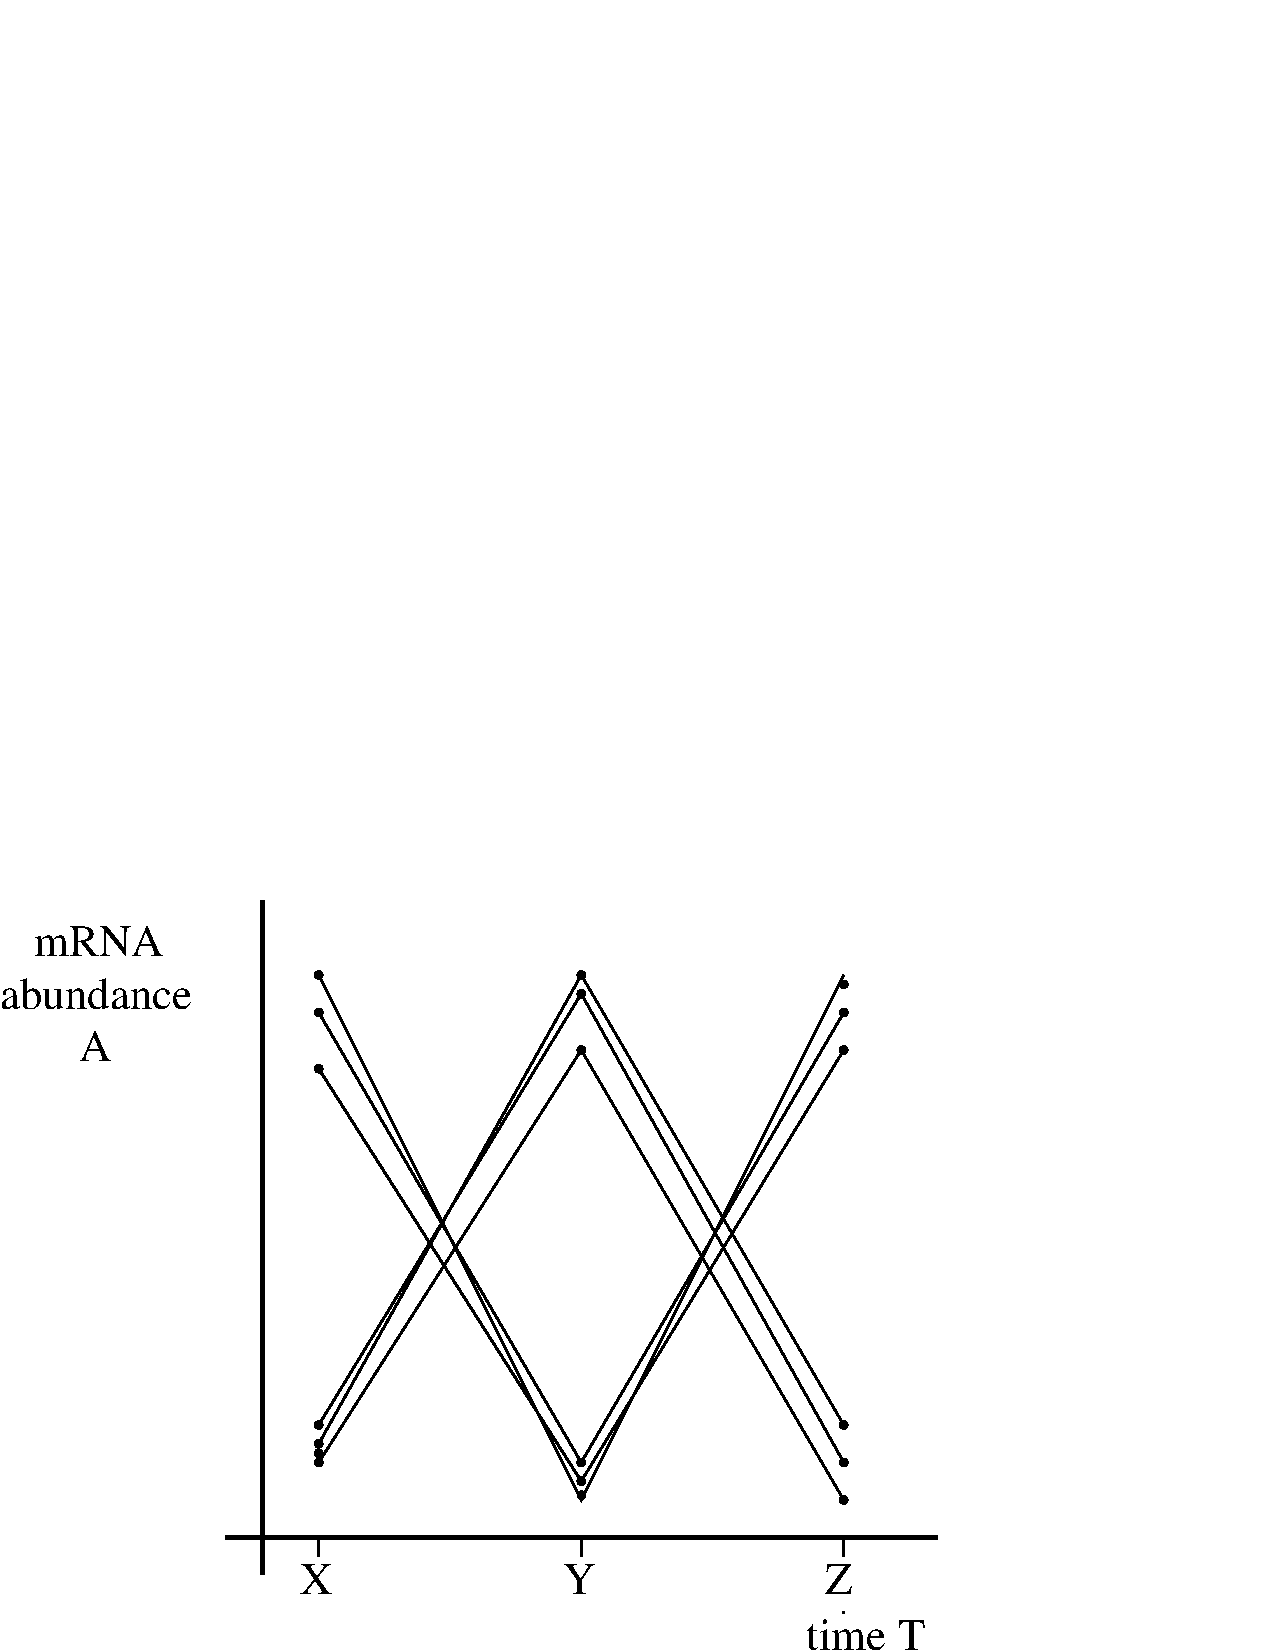
\includegraphics[height=0.4\textheight]{3d-data.pdf}
&
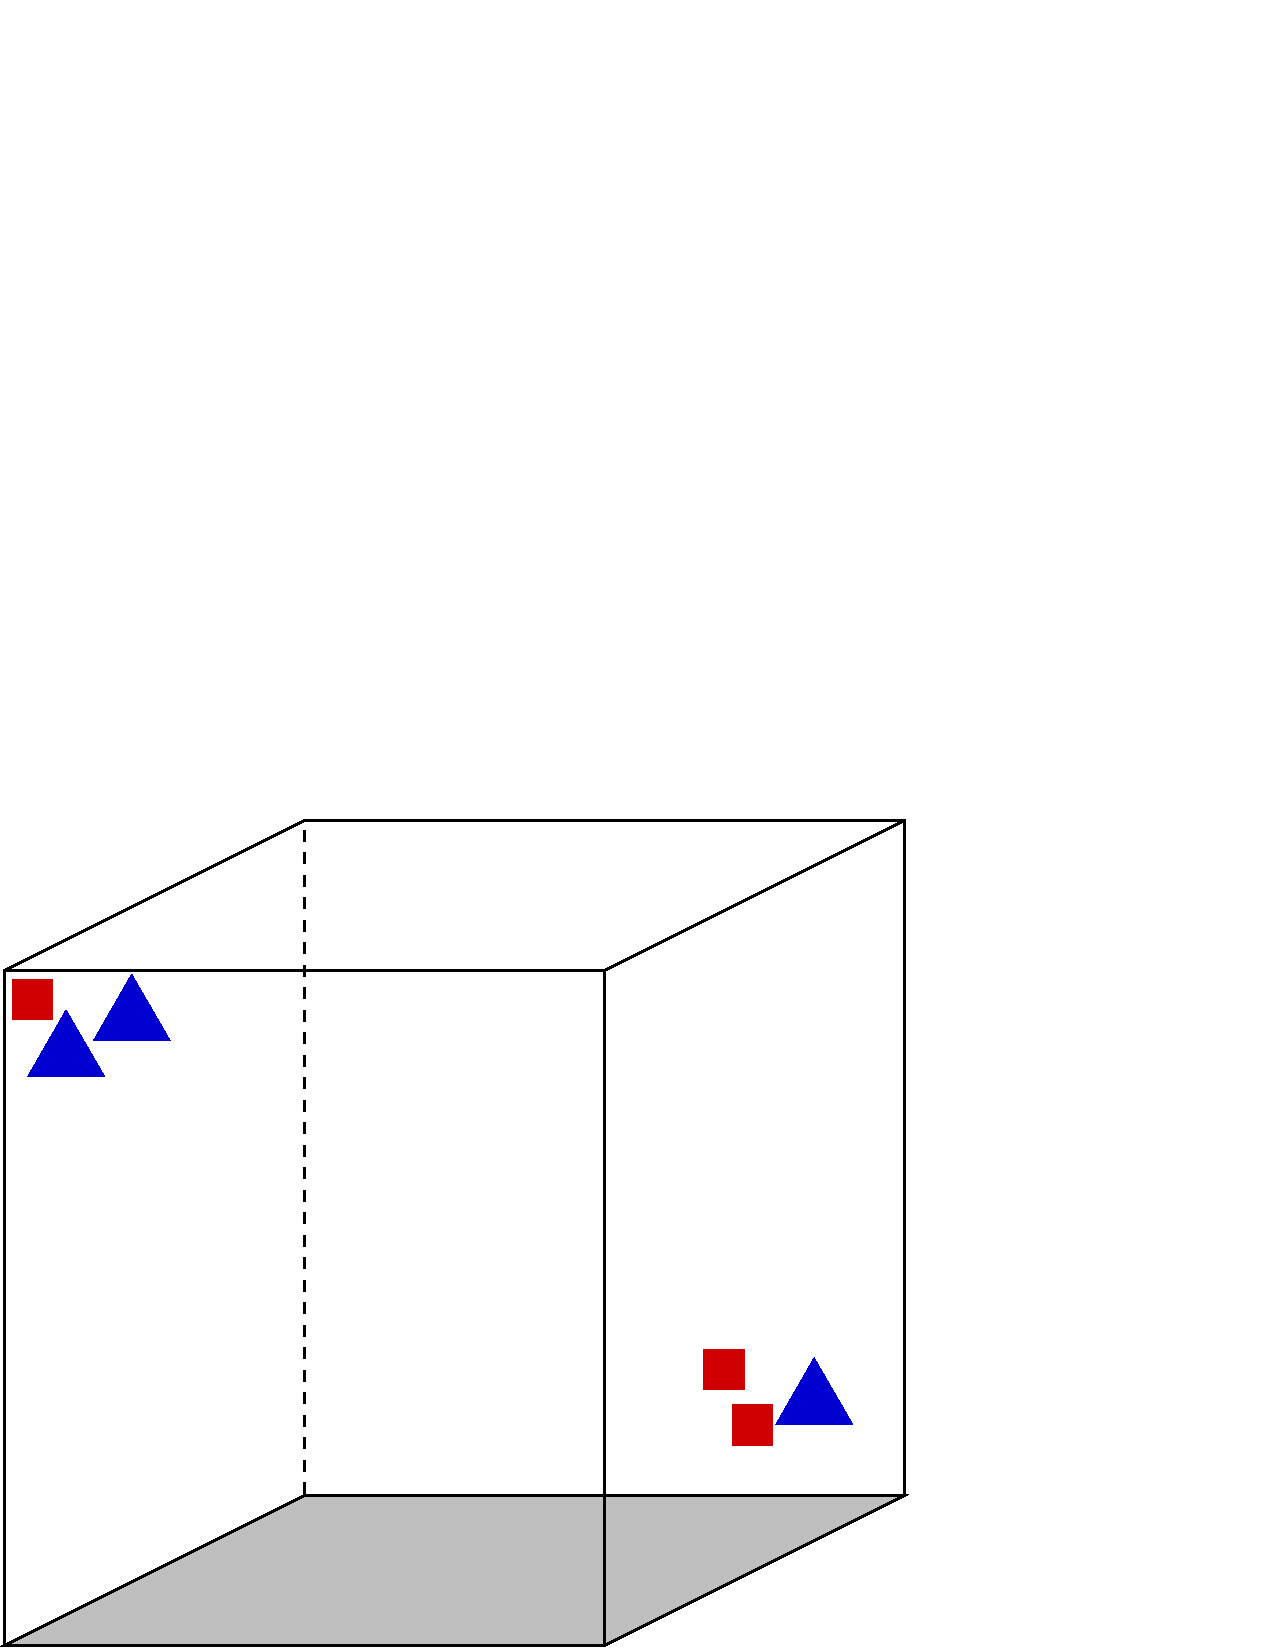
\includegraphics[height=0.4\textheight]{3d-kmeans1.pdf}
&
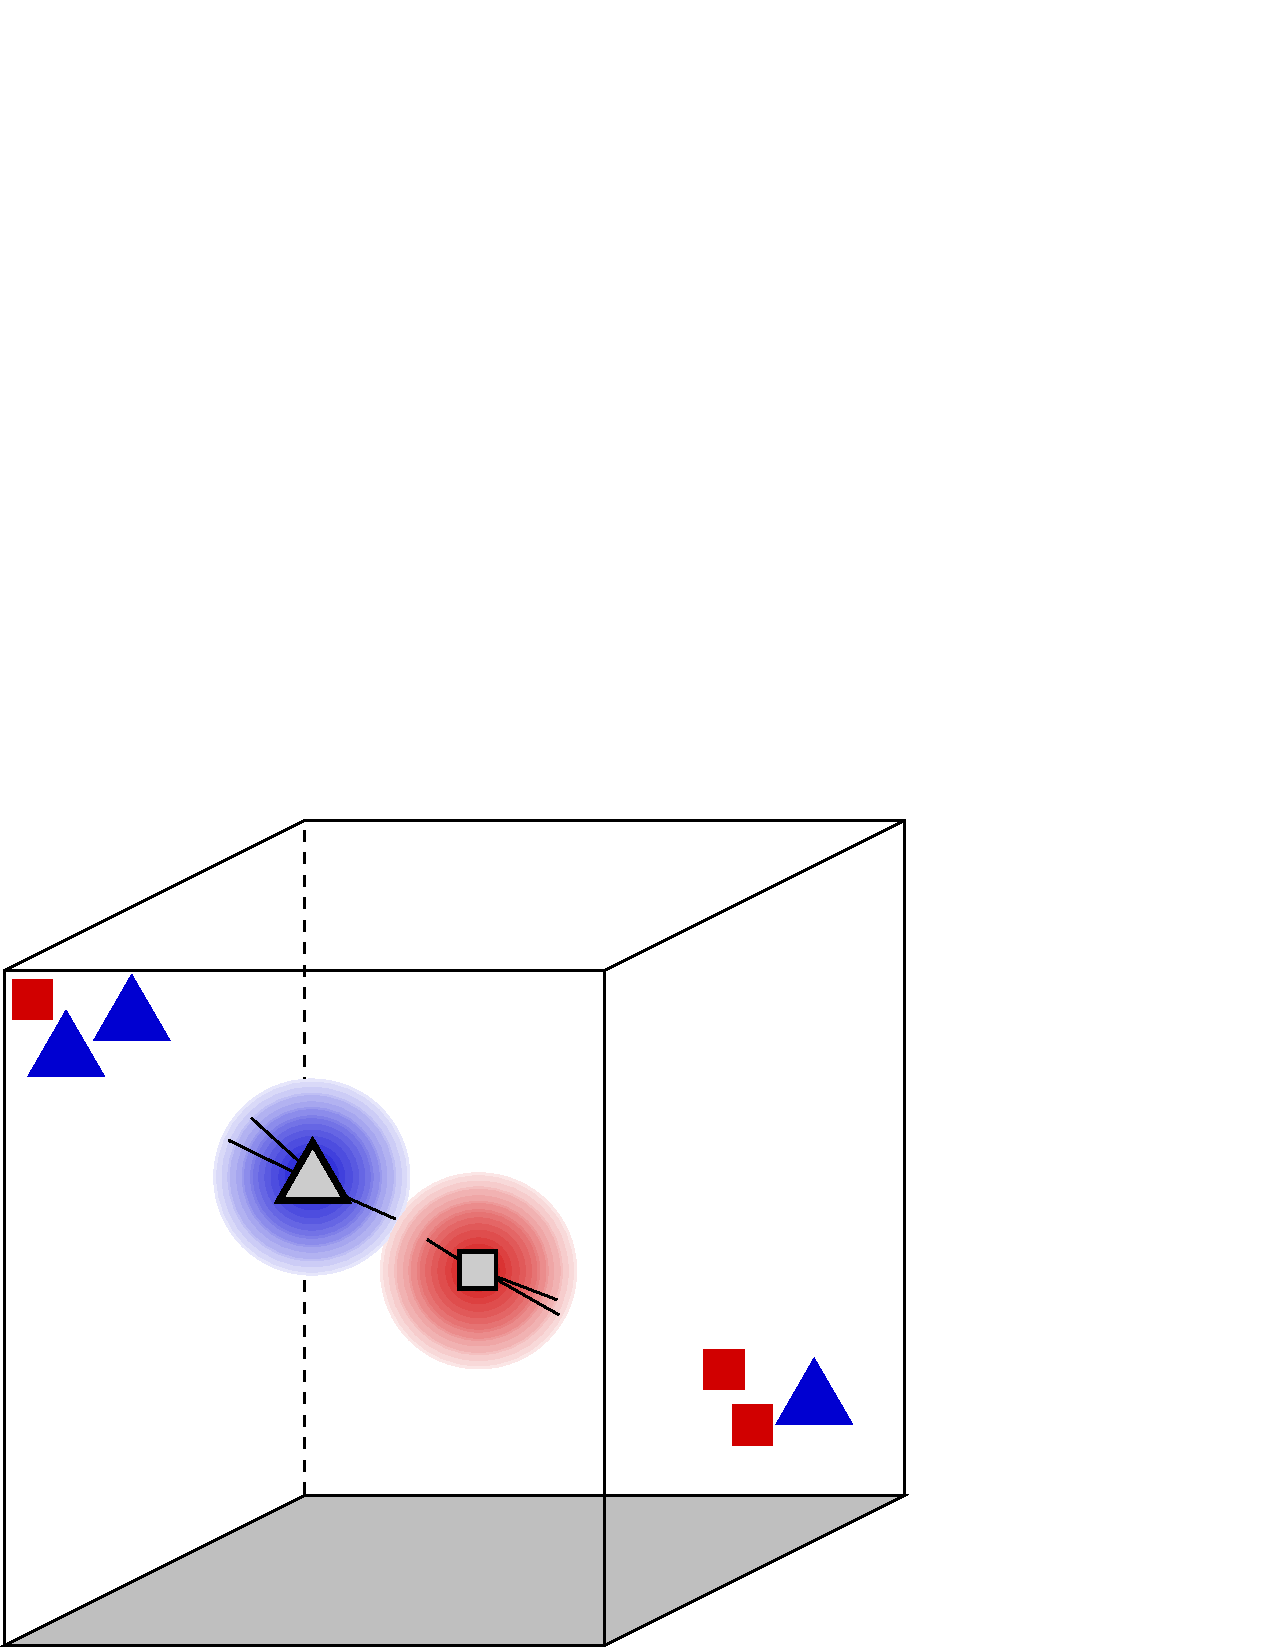
\includegraphics[height=0.4\textheight]{3d-kmeans2.pdf}
\\
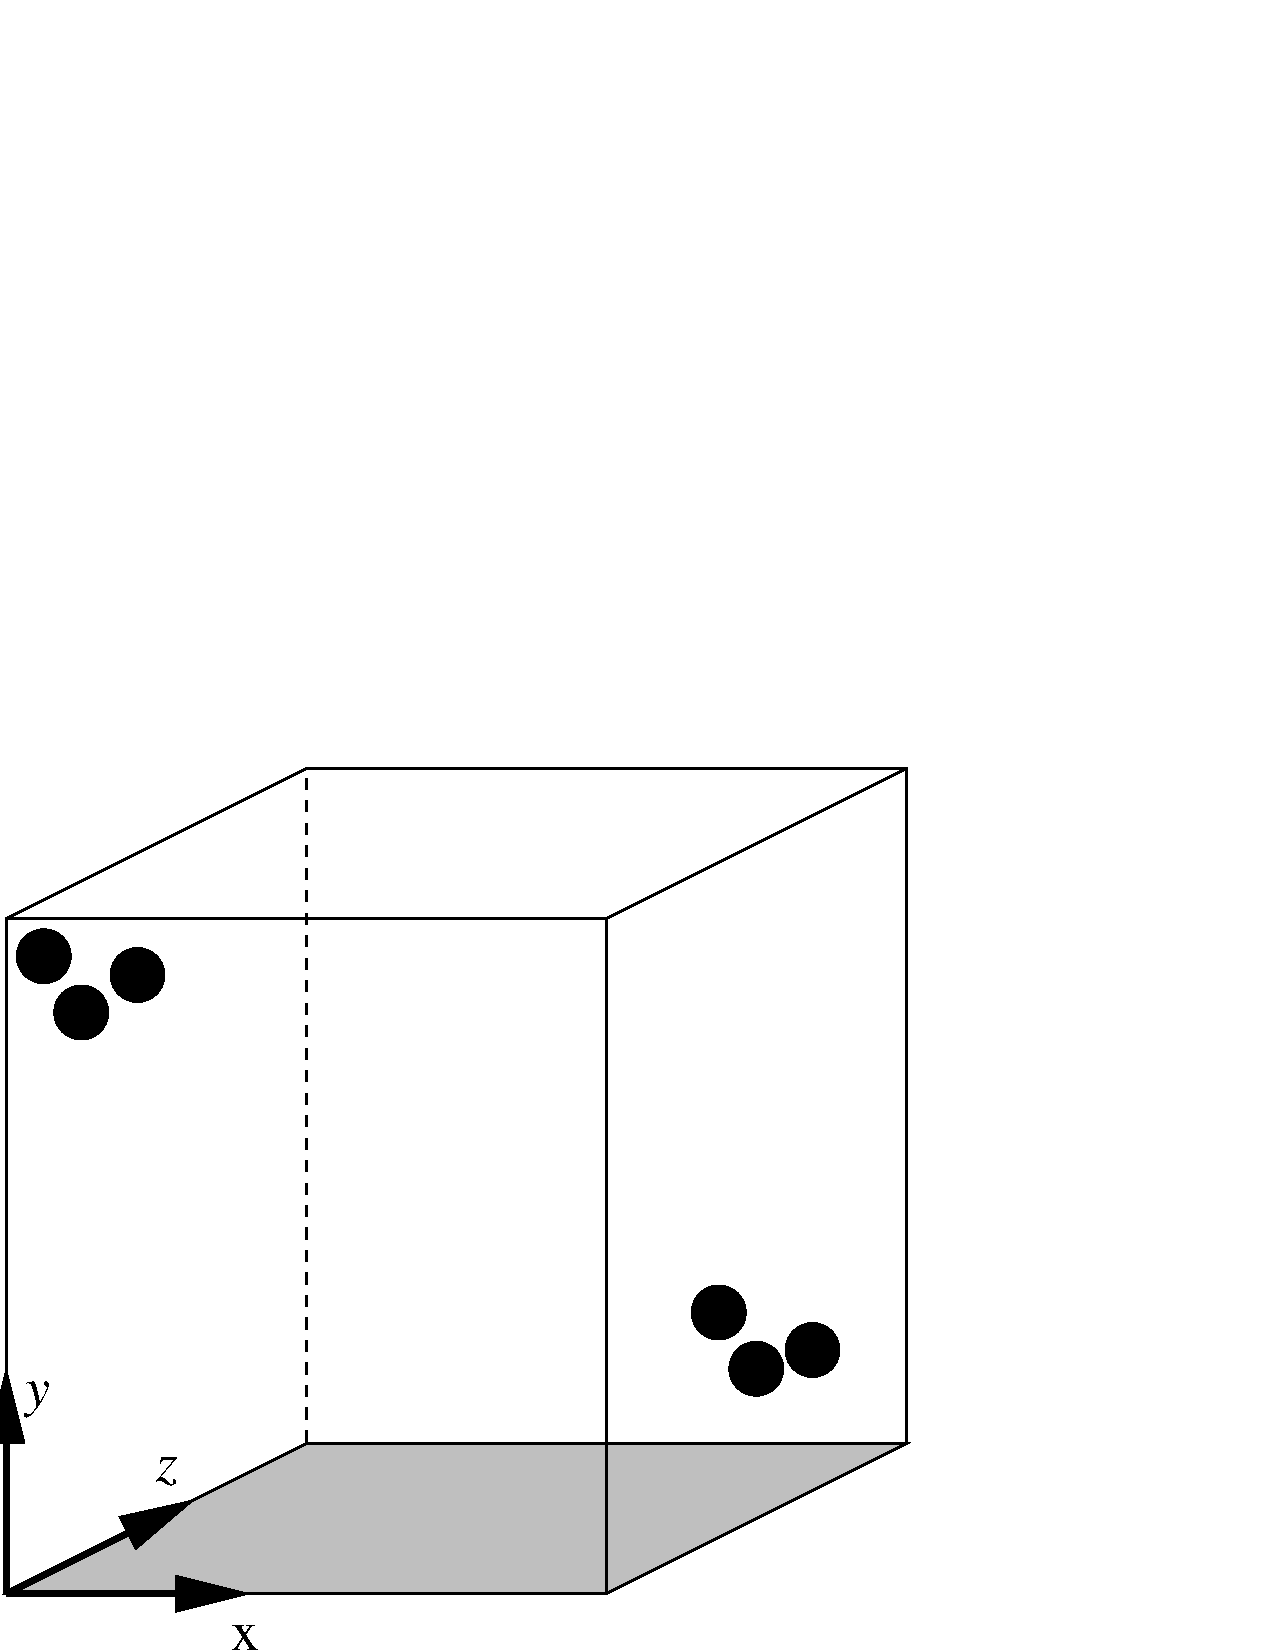
\includegraphics[height=0.4\textheight]{3d-data2.pdf}
&
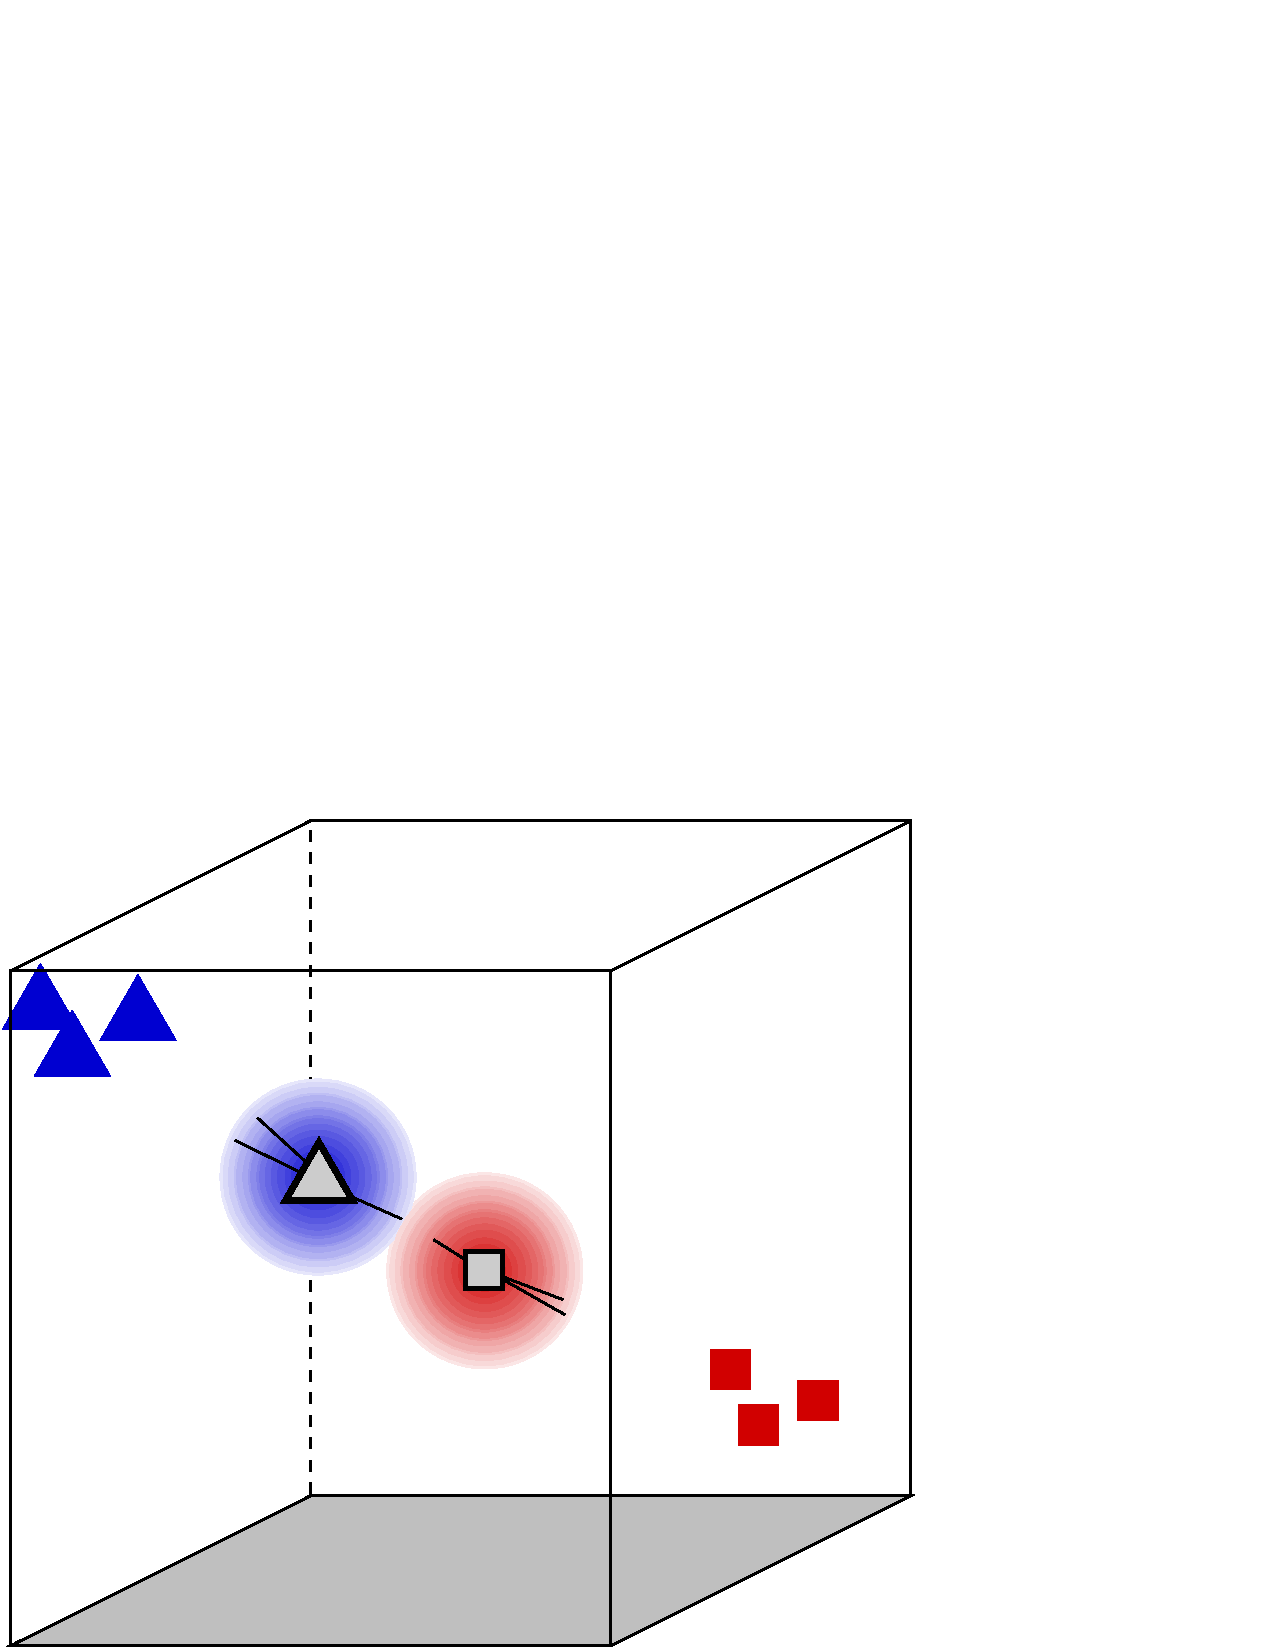
\includegraphics[height=0.4\textheight]{3d-kmeans3.pdf}
&
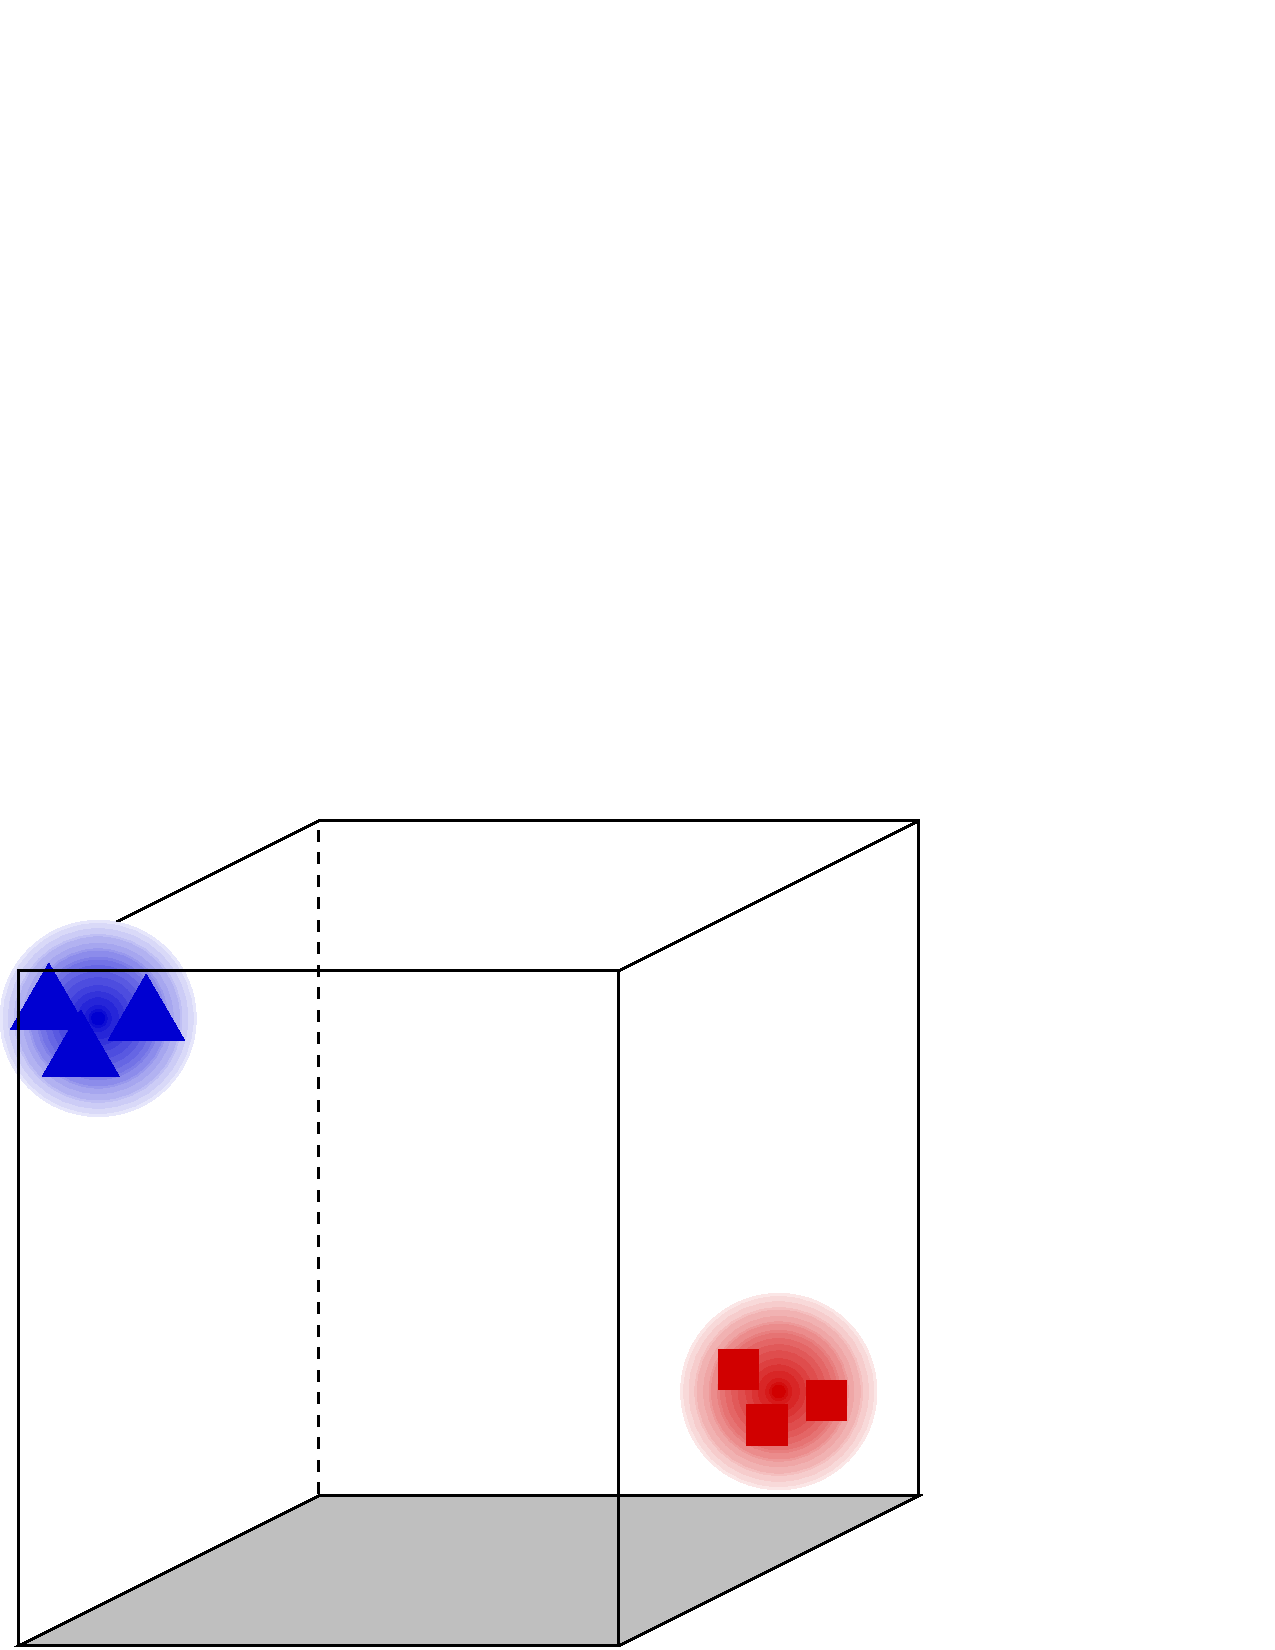
\includegraphics[height=0.4\textheight]{3d-kmeans4.pdf}
\end{tabular}

\end{frame}


\begin{frame}{Essence of the $K$-means algorithm}


Alternate between two steps
 \itemb
 \item Estimate {\em missing data} (cluster assignments)
 \item Estimate {\em model parameters} (cluster centroids)
 \iteme

\vspace{\baselineskip}

As we will see, this is very close in essence to EM.

\end{frame}

\begin{frame}{Variations on the $K$-means algorithm}

\itemb
\item ``$K$-medians'': use cluster medians instead of centroids (a bit more stable)
\item \alert{``Soft $K$-means'':} allow dataset$\to$cluster assignments to be probabilistic (``soft''), rather than deterministic (``hard'');
centroids are then probability-weighted averages
\iteme

We will see that soft $K$-means is, in fact, EM on a particular model.

\end{frame}


\section{Quick overview of EM}

\begin{frame}{What is the EM algorithm for?}

EM (Expectation-Maximization) is a very broad family of algorithms
for finding a \alert{maximum-likelihood point estimate} of some model parameters
\begin{eqnarray*}
\hat{\theta} & = & \argmax_{\theta} P(Y|\theta) \\
& = & \argmax_{\theta} \sum_X P(X,Y|\theta)
\end{eqnarray*}
where
\itemb
\item $X$ represents \alert{missing data} (unknown, to be summed out)
\item $Y$ represents \alert{observed data}
\iteme

\end{frame}


\begin{frame}{Characteristics of EM}

\itemb
\item Algorithm is \alert{iterative}
 \itemb
 \item Guaranteed to converge
 \item Convergence often rapid at first, then slow
 \iteme
\item Works for a lot of models (but not all)
\item Missing data ($X$) can often be summarized by \alert{counts}
\item Many generalizations (approximate, stochastic, etc.)
\iteme

\end{frame}


\begin{frame}{Formal statement of the EM algorithm}

\begin{eqnarray*}
\theta^{(n+1)} & = & \argmax_{\theta}\ {\cal E}(\theta|\theta^{(n)}) \\
{\cal E}(\theta|\theta^{(n)}) & = & \sum_x P(X|Y,\theta^{(n)}) \log P(X,Y|\theta) \\
& = & \langle \log P(X,Y|\theta) \rangle_{P(X|Y,\theta^{(n)})}
\end{eqnarray*}

\itemb
\item Find posterior of missing data, $P(X|Y,\theta^{(n)})$
\item Maximize expected log-likelihood under this posterior
\iteme

\end{frame}



\begin{frame}{Example: two-coin mixture}

\itemb
\item I have two coins, each of which has probability $p_k$ of returning heads and $q_k=1-p_k$ of tails ($k \in \{ 1,2 \}$)
\item We perform $E$ experiments.
\item In the $e$'th experiment, I pick one of the coins and flip it $F$ times, yielding $y_e$ heads and $z_e = F - y_e$ tails
\item Let $x_e$ be the coin I picked for the $e$'th experiment.
\item Missing data: $X = (x_1 \ldots x_E)$
\item Observed data: $Y = (y_1 \ldots y_E)$
\item Parameters: $\theta = (p_1, p_2)$
\iteme

\[
P(X,Y|\theta) = \prod_{e=1}^E \frac{1}{2} \binomial{F}{y_e} p_{x_e}^{y_e} q_{x_e}^{z_e}
\]

\end{frame}

\begin{frame}{EM algorithm for two-coin mixture}

First calculate the posterior distribution over $X|Y$ for given $\theta$

\begin{eqnarray*}
P(x_e=x,y_e=y|\theta) & = & \frac{1}{2} \binomial{F}{y} p_x^y q_x^z \\
P(y_e=y|\theta) & = & \sum_{x \in \{1,2\}} \frac{1}{2} \binomial{F}{y} p_x^y q_x^z \\
P(x_e=x|y_e=y,\theta) & = & P(x_e=x,y_e=y|\theta)\ /\ P(y_e=y|\theta) \\
& = & W_{e,x}
\end{eqnarray*}

where $z = F - y$

\end{frame}

\begin{frame}{EM algorithm for two-coin mixture}

Next write down the expected log-likelihood
\begin{eqnarray*}
\lefteqn{{\cal E}(\theta|\theta^{(n)})} \\
& = & \sum_X P(X|Y,\theta^{(n)}) \log P(X,Y|\theta) \\
% & = & \sum_X P(X|Y,\theta^{(n)}) \sum_e \log P(x_e,y_e|\theta) \\
% & = & \sum_e \sum_{x \in \{1,2\}} P(x_e=x|y_e,\theta^{(n)})  \log P(x_e=x,y_e|\theta) \\
& = & \sum_e \sum_{x \in \{1,2\}} W_{e,x} \left( y_e \log p_x + z_e \log q_x + K \right)
\end{eqnarray*}
where $K$ is independent of $\theta$
(it includes the binomial coefficient and the factor of $1/2$ corresponding to $P(x_e)$)
--- we can drop this term

\end{frame}

\begin{frame}{EM algorithm for two-coin mixture}

Here's a longer derivation of that
\begin{eqnarray*}
\lefteqn{{\cal E}(\theta|\theta^{(n)})} \\
& = & \sum_X P(X|Y,\theta^{(n)}) \log P(X,Y|\theta) \\
& = & \sum_X P(X|Y,\theta^{(n)}) \sum_e \log P(x_e,y_e|\theta) \\
& = & \sum_e \sum_{x \in \{1,2\}} P(x_e=x|y_e,\theta^{(n)})  \log P(x_e=x,y_e|\theta) \\
& = & \sum_e \sum_{x \in \{1,2\}} W_{e,x} \left( y_e \log p_x + z_e \log q_x + K \right)
\end{eqnarray*}

\end{frame}


\begin{frame}{EM algorithm for two-coin mixture}

\small
\[
{\cal E}(\theta|\theta^{(n)}) = \sum_{x \in \{1,2\}} \left[ \left( \sum_e W_{e,x} y_e \right) \log p_x + \left( \sum_e W_{e,x} z_e \right) \log q_x \right]
\]
\normalsize

\itemb
\item Experiment $e$ yielded $y_e$ heads and $z_e$ tails
\item Posterior probability that experiment $e$ used coin $x$ is $W_{e,x}$
\item For coin $x$, \alert{expected counts} are $h_x = \sum_e W_{e,x} y_e$ heads, $t_x = \sum_e W_{e,x} z_e$ tails, $f_x = h_x+t_x = \sum_e W_{e,x} F$ total flips
\iteme

Subject to probabilistic constraints on the $p_x$ the EM update is
\[
p_x \leftarrow \frac{h_x}{f_x}
\]

\end{frame}




\section{A closer look at EM}

\begin{frame}{Proof/derivation of EM}

 Following Anders Krogh (Durbin, Krogh {\em et al}, chapter 11.6)
  \itemb
  \item Suppose we have some estimate $\theta^{(n)}$ and we want to choose $\theta^{(n+1)}$ such that $P(y|\theta^{(n+1)}) \geq P(y|\theta^{(n)})$
  \item Since $P(x,y|\theta) = P(y|\theta) P(x|y,\theta)$ we can write $\log P(y|\theta) = \log P(x,y|\theta) - \log P(x|y,\theta)$ for some $\theta$
  \item Multiplying by $P(x|y,\theta^{(n)})$ and summing over $x$ gives
\begin{eqnarray*}
\lefteqn{\log P(y|\theta)} \\
& = & \sum_x P(x|y,\theta^{(n)}) \log P(x,y|\theta) - \sum_x P(x|y,\theta^{(n)}) \log P(x|y,\theta)
\end{eqnarray*}
 \iteme

\end{frame}

\begin{frame}{Derivation of EM}

\itemb
  \item Let first term on RHS be ${\cal E}(\theta|\theta^{(n)}) = \sum_x P(x|y,\theta^{(n)}) \log P(x,y|\theta)$. Then
\begin{eqnarray*}
\log P(y|\theta) & = & {\cal E}(\theta|\theta^{(n)}) - \sum_x P(x|y,\theta^{(n)}) \log P(x|y,\theta) \\
\log P(y|\theta^{(n)}) & = & {\cal E}(\theta^{(n)}|\theta^{(n)}) - \sum_x P(x|y,\theta^{(n)}) \log P(x|y,\theta^{(n)})
\end{eqnarray*}
  \item Subtracting gives
\begin{eqnarray*}
\lefteqn{\log P(y|\theta) - \log P(y|\theta^{(n)})} \\
& = & {\cal E}(\theta|\theta^{(n)}) - {\cal E}(\theta^{(n)}|\theta^{(n)}) + \sum_x P(x|y,\theta^{(n)}) \log \frac{P(x|y,\theta^{(n)})}{P(x|y,\theta)} \\
& = & {\cal E}(\theta|\theta^{(n)}) - {\cal E}(\theta^{(n)}|\theta^{(n)}) + D\left(P(x|y,\theta^{(n)}) || P(x|y,\theta)\right)
\end{eqnarray*}
 \iteme

\end{frame}

\begin{frame}{Proof of convergence of EM}

\begin{eqnarray*}
\lefteqn{\log P(y|\theta) - \log P(y|\theta^{(n)})} \\
& = & {\cal E}(\theta|\theta^{(n)}) - {\cal E}(\theta^{(n)}|\theta^{(n)}) + D\left(P(x|y,\theta^{(n)}) || P(x|y,\theta)\right)
\end{eqnarray*}

\itemb
  \item Since last term on RHS is always $\geq 0$, we have $P(y|\theta^{(n+1)}) \geq P(y|\theta^{(n)})$ as long as
\[
\theta^{(n+1)} = \argmax_{\theta}\ {\cal E}(\theta|\theta^{(n)})
\]
  \item If $\theta^{(n+1)} = \theta^{(n)}$, then a maximum has been reached and so $P(y|\theta^{(n+1)}) = P(y|\theta^{(n)})$
 \iteme

\end{frame}

\begin{frame}{Interpretation}

\itemb
  \item Again, ${\cal E}(\theta|\theta^{(n)})$ is the {\bf expected joint log-likelihood of the missing data $x$ and observed data $y$ as a function of $\theta$},
with the expectation taken over the posterior distribution of $x$ as estimated using $\theta^{(n)}$
  \item Computing $P(x|y,\theta^{(n)})$, or statistics that are sufficient to summarize this distribution, is called the {\bf E-step} of EM.
  \item Computing $\theta^{(n+1)} = \argmax_{\theta} {\cal E}(\theta|\theta^{(n)})$ is the {\bf M-step} of EM.
 \iteme

\end{frame}

\begin{frame}{Expected counts}

Note if $P(x,y|\theta)$ has the form $\prod_i \theta_i^{x_i}$,
where $x_i$ is the number of times an event occurs and $\theta_i$ is the probability of that event,
then ${\cal E}(\theta|\theta^{(n)})$ has the form $\sum_i \expect{x_i}_{P(x|y,\theta^{(n)})} \log \theta_i$

   \itemb
   \item ${\cal E}$ typically involves {\bf expected counts} $\expect{x_i}$ for missing data
\itemb
   \item In this case, EM is making use of the first derivatives:
\begin{eqnarray*}
\pderiv{(\log P(y|\theta))}{(\log \theta_i)} & = & \frac{\theta_i}{P(y|\theta)} \pderiv{P(y|\theta)}{\theta_i} \\
 & = & \frac{\theta_i}{P(y|\theta)} \pderivop{\theta_i} \sum_x P(x,y|\theta) \\
 & = & \frac{\theta_i}{P(y|\theta)} \sum_x \left( \frac{x_i}{\theta_i} \right) P(x,y|\theta) \\
 & = & \frac{\theta_i}{P(y|\theta)} \sum_x \left( \frac{x_i}{\theta_i} \right) P(y|\theta) P(x|y,\theta)
= \expect{x_i}_{P(x|y,\theta)}
\end{eqnarray*}
   \iteme
\iteme

\end{frame}

\begin{frame}{Expected wait times}

\itemb
  \item Likewise if $P(x,y|\theta)$ contains terms of the form $\exp(-\theta_i x_i)$, where $\theta_i$ is an event rate and $x_i$ is the time that elapses before the event occurs,
the corresponding terms in ${\cal E}$ will be $-\theta_i \expect{x_i}$ involving the {\bf expected wait times} $\expect{x_i}$
  \iteme

\end{frame}

\begin{frame}{Neal and Hinton's variational view of EM}

\itemb
 \item Neal \& Hinton (Learning in Graphical Models, Jordan, 1998)
  \itemb
  \item Let $\tilde{P}(x)$ be a probability distribution over the missing data and let $H(\tilde{P})$ be the entropy of $\tilde{P}$. Define
\begin{eqnarray*}
F(\theta,\tilde{P}) & = & \expect{\log P(x,y|\theta)}_{\tilde{P}} + H(\tilde{P}) \\
& = & \sum_x \tilde{P}(x) \left( \log P(x,y|\theta) - \log \tilde{P}(x) \right) \\
& = & \sum_x \tilde{P}(x) \left( \log P(y|\theta) + \log P(x|y,\theta) - \log \tilde{P}(x) \right) \\
& = & \log P(y|\theta) - D \left( \tilde{P}(x)||P(x|y,\theta) \right)
\end{eqnarray*}
where $D(\tilde{P}(x)||P(x,y,\theta))$ is the relative entropy.
  \iteme
 \iteme

\end{frame}

\begin{frame}{Neal and Hinton's variational view of EM}

\[
F(\theta,\tilde{P}) = \expect{\log P(x,y|\theta)}_{\tilde{P}} + H(\tilde{P}) = \log P(y|\theta) - D \left( \tilde{P}(x)||P(x|y,\theta) \right)
\]

\itemb
  \item Suppose we fix $\theta=\theta^{(n)}$ and maximise $F(\theta^{(n)},\tilde{P})$ w.r.t. $\tilde{P}$.
Then the latter expression for $F$ shows that the maximum is at $\tilde{P}(x) = P(x|y,\theta^{(n)})$ (due to Gibbs' inequality).
This is the $E$-step of EM.
  \item If we then fix $\tilde{P}$ at this value, we have $F(\theta,\tilde{P})=F(\theta,P(x|y,\theta^{(n)})) = {\cal E}(\theta|\theta^{(n)}) + H(\tilde{P})$.
Maximising this w.r.t. $\theta$ is the M-step of EM.
  \item Thus EM can be viewed as a two-step maximization of $F$.
If $\left[-\log P(x,y|\theta)\right]$ is analogous to the ``energy'' of state $x$, then $[-F]$ is like a ``free energy'' (energy minus entropy).
 \iteme

\end{frame}


\section{Applications of EM}

\begin{frame}{Specific examples of EM}

We will look at two specific examples of how EM can be applied:
\itemb
\item EM on a mixture of Gaussians (``soft $K$-means'')
\inone{for clustering general multi-dimensional data}
\item EM on a continuous-time finite-state Markov chain (``phylo-EM'')
\inone{for estimating a substitution model from aligned sequence data}
\iteme

\end{frame}

\begin{frame}{$K$-means again}

Mixture-of-Gaussians example
 \itemb
 \item Again, suppose we have $N$ datapoints $\{y_i\}$ (restricted to one dimension for simplicity)
 \item Probabilistic model: mixture of $K$ Gaussian components; component $k$ has mean $m_k$ and variance $v_k$.
Parameters $\theta = \{ m_k, v_k \}$.
Each component has equal probability $1/K$.
\iteme

\end{frame}

\begin{frame}{Mixture of Gaussians: likelihoods}

\itemb
 \item If component label of point $i$ is $x_i$, then joint likelihood for point $i$ is
\[
P(x_i,y_i|\theta) = \frac{1}{K} (2\pi v_{x_i})^{-\frac{1}{2}} \exp(-\frac{1}{2}(y_i-m_{x_i})^2/v_{x_i})
\]
 \item Marginal likelihood for observed data is
\[
P(y_i|\theta) = \sum_{x_i} P(x_i,y_i|\theta)
\]
 \item Joint likelihood for all observed data and missing component labels is
\[
P(x,y|\theta) = \prod_{i=1}^N P(x_i,y_i|\theta)
\]
\iteme

\end{frame}

\begin{frame}{Posterior expectations}

\itemb
 \item Posterior probability of $i$'th component label (the E-step) is
\[
P(x_i|y_i,\theta) = \frac{P(x_i,y_i|\theta)}{P(y_i|\theta)}
\]
 \item Expected log-likelihood: let $W_i(x_i) = P(x_i|y_i,\theta^{(n)})$. Then
\begin{eqnarray*}
{\cal E}(\theta|\theta^{(n)}) & = & \expect{\log P(x,y|\theta)}_{P(x|y,\theta^{(n)})} \\
& = & \sum_{i=1}^N \expect{\log P(x_i,y_i|\theta)}_{P(x_i|y_i,\theta^{(n)})} \\
& = & -N \log K - \frac{N}{2} \log (2\pi) \\
& & - \frac{1}{2} \sum_{i=1}^N \sum_{k=1}^K W_i(k) \left( \log (v_k) + \frac{(y_i-m_k)^2}{v_k} \right) \\
\end{eqnarray*}
\iteme
\end{frame}

\begin{frame}{Deriving $K$-means}

\begin{eqnarray*}
{\cal E}(\theta|\theta^{(n)}) & = &  -N \log K - \frac{N}{2} \log (2\pi) \\
& & - \frac{1}{2} \sum_{i=1}^N \sum_{k=1}^K W_i(k) \left( \log (v_k) + \frac{(y_i-m_k)^2}{v_k} \right) \\
\end{eqnarray*}

Partial derivatives of ${\cal E}(\theta|\theta^{(n)})$
\begin{eqnarray*}
\pderiv{{\cal E}}{m_k} & = & \sum_{i=1}^N W_i(k) \frac{y_i - m_k}{v_k} \\
\pderiv{{\cal E}}{v_k} & = & -\frac{1}{2} \sum_{i=1}^N W_i(k) \left( \frac{1}{v_k} - \frac{(y_i-m_k)^2}{v_k^2} \right)
\end{eqnarray*}

\end{frame}

\begin{frame}{(Soft) $K$-means recovered}

\itemb
 \item Setting the partial derivatives to zero gives
\begin{eqnarray*}
m_k & = & \frac{\sum_i W_i(k) y_i}{\sum_i W_i(k)} \\
v_k & = & \frac{\sum_i W_i(k) (y_i - m_k)^2}{\sum_i W_i(k)} \\
& = & \frac{\sum_i W_i(k) y_i^2}{\sum_i W_i(k)} - \left( \frac{\sum_i W_i(k) y_i}{\sum_i W_i(k)} \right)^2
\end{eqnarray*}
which are immediately recognisable as the mean and variance of the $y_i$, weighted by $W_i(k)$.
\item As variance $\to$ 0, ``soft'' $K$-means becomes ``hard'' $K$-means
\iteme
\end{frame}

\begin{frame}{Notes on soft $K$-means}

\itemb
 \item The original $K$-means algorithm is equivalent to (a) only estimating the $m_k$ and (b) taking the limit $v_k \to 0\ \forall\ k$ so that $W_i(k) \to 1$ for the most probable cluster and $0$ for all other clusters.
Neal and Hinton refer to this as a ``winner-take-all'' variant of EM. It's also called ``hard'' (vs ``soft'') $K$-means.
 \item Note that soft $K$-means can get stuck in an infinite-likelihood ``trap'' if a single point gets assigned to a cluster and $v_k \to 0$.
This can be fixed by putting a prior distribution on the parameters $(m_k,v_k)$.
 \item Works on pretty much any mixture (not just Gaussians)
\iteme
% Algorithms that make use of second derivatives (indirectly or directly): conjugate gradient, quasi-Newton, Gauss-Newton, Newton-Raphson...
% http://www.faqs.org/faqs/ai-faq/neural-nets/part2/section-5.html

\end{frame}


\begin{frame}{Substitution models}

Short-time approximation (Dayhoff {\em et al})
\itemb
\item take a pairwise alignment of two closely related sequences
\item count the number of instances $C_{ij}$ of each aligned residue-pair $(i,j)$
\item estimate the evolutionary distance $\Delta t$ separating the two sequences
\item set $R_{ij} \leftarrow C_{ij} / \Delta t$.
\iteme
\end{frame}

\begin{frame}{Beyond the short-time approximation}
 \itemb
 \item Drawback: ignores multiple substitutions. We seek a maximum likelihood version,
with the likelihood implicitly taking multiple substitutions into account.
 \item We will see that this amounts (at least for the discrete-time approximation)
to getting an ``unbiased'' estimate of ${\bf C}$.
These correspond to the {\em expected} number of times that each $i \to j$ transition occurred.
 \item Our unbiased estimate of ${\bf C}$ depends on our current estimate of the rate matrix:
if we think that the $R_{ij}$ are small, there will be few multiple substitutions,
but if the $R_{ij}$ are large, there will be many.
Thus the two things that we are trying to estimate are inter-related, but that's how EM works:
we fix one and estimate the other, then do it the other way round, then iterate to convergence.
 \iteme
\end{frame}

\begin{frame}{Beyond the short-time approximation}
 \itemb
 \item We start with a discrete-time approximation (breaking the time interval into small, finite steps).
We then consider the limit where the time-steps get infinitely small.
In this continuous-time limit, there are an infinite number of $i \to i$ transitions.
It then makes more sense to consider the amount of {\em time} spent in state $i$.
\item Take the pairwise case first.
The derivation is laborious but the result we're aiming for is that we can get our expected counts ${\bf C}$
by conditioning on, then summing over, all possible times at which a substitution can occur.
 \iteme
\end{frame}

\begin{frame}{Discrete-timestep version}
 \itemb
 \item Use discrete-time approximation: break $T$ into discrete steps of size $\Delta t$
with discrete-time transition matrix ${\bf Q} = {\bf I} + {\bf R} \Delta t$
(later we'll take limit $\Delta t \to 0$).
Let $x_n$ be the state at time $t = n \Delta t$.
Let the p.d.f. over $x_0$ be $\pi_{x_0}$.
Suppose that $x_0=a$ and $x_N=b$ are observed (where $N = T / \Delta t$),
while states $x_1 \ldots x_{N-1}$ are missing data.
Thus
\begin{eqnarray*}
P(x_0 \ldots x_N | \theta) & = & \pi_{x_0} \prod_{n=0}^{N-1} Q_{x_n x_{n+1}} \\
P(x_0, x_N | \theta) & = & \pi_{x_0} \left[ {\bf Q}^N \right]_{x_0 x_N} \\
\displaystyle
P(x_1 \ldots x_{N-1} | x_0, x_N, \theta) & = & \frac{P(x_0 \ldots x_N | \theta)}{P(x_0, x_N | \theta)}
\end{eqnarray*}
 \iteme
\end{frame}

\begin{frame}{Expected transition counts}
 \itemb
 \item Let $\theta' = (\pi', {\bf Q}')$ be the old parameters and $\theta = (\pi, {\bf Q})$ be the new parameters.
The EM function ${\cal E}(\theta|\theta')$ is
\[
{\cal E}(\theta|\theta') = \log \pi_{x_0} + \sum_i \sum_j C_{ij} \log Q_{ij}
\]
where $C_{ij}$ is the {\bf expected number of times that the transition $i \to j$ occurred.}
This can be seen immediately from the fact that the joint likelihood for observed \& missing data can be written in the form
\[
P(x_0 \ldots x_N | \theta) = \pi_{x_0} \prod_i \prod_j Q_{ij}^{\xi_{ij}}
\]
where $\xi_{ij}$ counts the usage of transition $i \to j$. \\
Then we can deduce that $C_{ij} = \expect{\xi_{ij}}$.
 \iteme
\end{frame}

\begin{frame}{A longer derivation}

\tiny
\begin{eqnarray*}
{\cal E}(\theta|\theta')
& = & \sum_{x_1} \sum_{x_2} \ldots \sum_{x_{N-1}} P(x_1 \ldots x_{N-1} | x_0, x_N, \theta') \log P(x_0 \ldots x_N | \theta) \\
%& = & \sum_{x_1} \sum_{x_2} \ldots \sum_{x_{N-1}} P(x_1 \ldots x_{N-1} | x_0, x_N, \theta') \log \left( \pi_{x_0} \prod_{n=0}^{N-1} Q_{x_n x_{n+1}} \right) \\
& = & \sum_{x_1} \sum_{x_2} \ldots \sum_{x_{N-1}} P(x_1 \ldots x_{N-1} | x_0, x_N, \theta') \left( \log \pi_{x_0} + \sum_{n=0}^{N-1} \log Q_{x_n x_{n+1}} \right) \\
& = & \log \pi_{x_0} + \sum_{n=0}^{N-1} \sum_{x_n} \sum_{x_{n+1}}
\left[ \sum_{\{x_k:\ 1 \leq k < n,\ n+1 < k \leq N\}} P(x_1 \ldots x_{N-1} | x_0, x_N, \theta') \right]
\log Q_{x_n x_{n+1}} \\
& = & \log \pi_{x_0} + \sum_{n=0}^{N-1} \sum_{x_n} \sum_{x_{n+1}}
\left[ \notsum{x_n,x_{n+1}} P(x_1 \ldots x_{N-1} | x_0, x_N, \theta') \right]
\log Q_{x_n x_{n+1}} \\
& = & \log \pi_{x_0} +\sum_{n=0}^{N-1} \sum_{x_n} \sum_{x_{n+1}} P(x_n,x_{n+1}|x_0,x_N,\theta') \log Q_{x_n x_{n+1}} \\
& = & \log \pi_{x_0} + \sum_i \sum_j \left[ \sum_{n=0}^{N-1} P(x_n=i,x_{n+1}=j|x_0,x_N,\theta') \right] \log Q_{ij} \\
& = & \log \pi_{x_0} + \sum_i \sum_j C_{ij} \log Q_{ij}
\end{eqnarray*}
\end{frame}

\begin{frame}{Calculating the expected transition counts}

$C_{ij}$ is the expected number of transitions $i \to j$ that occurred among the missing data.
Recalling that the start and end states are $x_0=a$ and $x_N=b$,
and observing that the expectation $C_{ij}$ is additive over all timepoints $n$ at which the transition could occur,
we have
\small
\begin{eqnarray*}
C_{ij} & = & \sum_{n=0}^{N-1} P(x_n=i,x_{n+1}=j|x_0=a,x_N=b,\theta') \\
& = & \sum_{n=0}^{N-1} \frac{P(x_n=i|x_0=a,\theta') P(x_{n+1}=j|x_n=i,\theta') P(x_N=b|x_{n+1}=j,\theta')}{P(x_N=b|x_0=a,\theta')} \\
& = & \sum_{n=0}^{N-1} \frac{[{\bf Q}^n]_{ai} Q_{ij} [{\bf Q}^{N-n-1}]_{jb}}{[{\bf Q}^N]_{ab}}
\end{eqnarray*}
\end{frame}

\begin{frame}{Summary so far}

So far we have the counts in terms of something like a convolution of two matrix exponentials

\[
C_{ij} = \frac{Q_{ij}}{[{\bf Q}^N]_{ab}} \sum_{n=0}^{N-1} [{\bf Q}^n]_{ai} [{\bf Q}^{N-n-1}]_{jb}
\]

We can get explicit forms for terms like $[{\bf Q}^n]_{ai}$ using the diagonalized matrix form.

\end{frame}

\begin{frame}{Eigenform of transition counts}
Eigenvector decomposition ${\bf Q} = {\bf UDU}^{-1}$, where ${\bf D}$ is diagonal (with $D_{kk} = \lambda_k$),
gives us ${\bf Q}^n = {\bf UD}^n {\bf U}^{-1}$ and so
\begin{eqnarray*}
C_{ij} & = & \frac{Q_{ij}}{[{\bf UD}^N {\bf U}^{-1}]_{ab}}
\sum_{n=0}^{N-1} [{\bf UD}^n {\bf U}^{-1}]_{ai} [{\bf UD}^{N-n-1} {\bf U}^{-1}]_{jb} \\
& = & \frac{Q_{ij}}{\sum_m U_{am} \lambda^N_m U^{-1}_{mb}} \sum_{n=0}^{N-1}
\left( \sum_k U_{ak} \lambda_k^n U^{-1}_{ki} \right)
\left( \sum_l U_{jl} \lambda_l^{N-n-1} U^{-1}_{lb} \right) \\
& = & \frac{Q_{ij}}{\sum_m U_{am} \lambda^N_m U^{-1}_{mb}}
\sum_k U_{ak} U^{-1}_{ki} \sum_l U_{jl} U^{-1}_{lb}
\sum_{n=0}^{N-1} \lambda_k^n \lambda_l^{N-n-1}
\end{eqnarray*}
\end{frame}

\begin{frame}{Eigenvector interaction matrix}
\begin{eqnarray*}
C_{ij} & = & \frac{Q_{ij}}{\sum_m U_{am} \lambda^N_m U^{-1}_{mb}}
\sum_k U_{ak} U^{-1}_{ki} \sum_l U_{jl} U^{-1}_{lb}
\sum_{n=0}^{N-1} \lambda_k^n \lambda_l^{N-n-1}  \\
& = & \frac{Q_{ij}}{\sum_m U_{am} \lambda^N_m U^{-1}_{mb}}
\sum_k U_{ak} U^{-1}_{ki} \sum_l U_{jl} U^{-1}_{lb} \Lambda_{kl}
\end{eqnarray*}
where
\[
\Lambda_{kl} = \left\{ \begin{array}{ll}
\displaystyle
\frac{\lambda_l^N - \lambda_k^N}{\lambda_l - \lambda_k} & \mbox{if $\lambda_k \neq \lambda_l$} \\
N \lambda_l^{N-1} & \mbox{if $\lambda_k = \lambda_l$}
\end{array} \right.
\]
To obtain $\Lambda_{kl}$ we have used the identity $\sum_{k=0}^{N-1} a^k = (a^N - 1)/(a-1)$.
\end{frame}

\begin{frame}{From one column to an alignment}

So far we've estimated a summary of the missing data for a single column of an alignment.

Hopefully it should also be clear that if we have two sequences $X,Y$ of length $L$ then the expected counts matrix ${\bf C}$
can be obtained by summing over all sites $X_l,Y_l$, so
\[
C_{ij} = \sum_{l=1}^L C_{ij}^{[X_l \stackrel{N}{\to} Y_l]}
\]
where $C_{ij}^{[a \stackrel{N}{\to} b]}$ is the $C_{ij}$ derived above for a process beginning in state $x_0=a$ and ending in $x_N=b$.
\end{frame}

\begin{frame}{Discrete-timestep EM algorithm}
 \itemb
 \item To summarise: the EM algorithm for parameterising a discrete-time Markov chain from a pairwise alignment is
  \enumb
  \item Start with some initial estimate of the probability matrix ${\bf Q}$.
  \item Estimate the transition counts $C_{ij}$ by summing over all sites $X_l,Y_l$ as above.
  \item Update $Q_{ij} \leftarrow C_{ij} / \sum_k C_{ik}$ (that this maximizes ${\cal E}$ can be seen using Lagrange multipliers)
  \item Repeat until the algorithm converges on a fixed matrix ${\bf Q}$ (i.e. until the likelihood $P(Y|X,{\bf Q})$ stabilises).
  \enume
\iteme
\end{frame}

\begin{frame}{From discrete to continuous}
 \itemb
\item Continuous limit: as $\Delta t \to 0$, so $N \to \infty$.
The upshot of this is that $C_{ij}$ converges and is meaningful for $i \neq j$, but $C_{ii} \sim 1/N \to \infty$
because during most of the short time intervals, the chain stays in the same state.
 \itemb
 \item More detailed argument: the $N$-dependent terms in the expression for $C_{ij}$
are $Q_{ij} \Lambda_{kl} / {\bf Q}^N_{ab}$
with $Q_{ij} = \delta_{ij} + R_{ij}/N$.
The factors of $\lambda^N$ approximately cancel in $\Lambda_{kl}$ and ${\bf Q}^N_{ab}$,
and the factor of $N$ in $\Lambda_{kk}$ cancels the $1/N$ in $Q_{ij}$ as long as $i \neq j$.
However, when $i=j$, there is an unaccounted factor of $N$ from $\Lambda_{kk}$
(indeed from all $\Lambda_{kl}$ where $\lambda_k = \lambda_l$).
 \item To get round this, we can define $W_i = C_{ii} T/N = C_{ii} \Delta t$ to be the expected {\em time} spent waiting in state $i$.
This then converges to a meaningful, finite value as $\Delta t \to 0$.
\iteme
\iteme
\end{frame}

\begin{frame}{Continuous-time transition counts and wait times}
\tiny
Since ${\bf M}(t) = \exp({\bf R}t)$, by analogy to the discrete case
\begin{eqnarray*}
C_{ij} & = & \frac{1}{M(T)_{ab}} \int_0^T M(t)_{ai} (R_{ij} dt) M(T-t)_{jb} \\
& = & \frac{R_{ij}}{\sum_m U_{am} \exp(\lambda_m T) U^{-1}_{mb}}
\sum_k U_{ak} U^{-1}_{ki} \sum_l U_{jl} U^{-1}_{lb} {\cal J}_{kl}(T) \\
W_i & = & \frac{1}{M(T)_{ab}} \int_0^T M(t)_{ai} (dt) M(T-t)_{jb} \\
& = & \frac{1}{\sum_m U_{am} \exp(\lambda_m T) U^{-1}_{mb}} \sum_k U_{ak} U^{-1}_{ki} \sum_l U_{jl} U^{-1}_{lb} {\cal J}_{kl}(T)
\end{eqnarray*}
where
\[
{\cal J}_{kl}(T) = \int_0^T \exp(\lambda_k t) \exp (\lambda_l(T-t)) dt = \left\{ \begin{array}{ll}
\displaystyle
\frac{\exp(\lambda_l T) - \exp(\lambda_k T)}{\lambda_l - \lambda_k} & \mbox{if $\lambda_k \neq \lambda_l$} \\
T \exp(\lambda_k T) & \mbox{if $\lambda_k = \lambda_l$}
\end{array} \right.
\]
\itemb
 \item The estimates for $C_{ij}$ and $W_i$ can be tested by simulation.
 \item The $\lambda_k$ in the above expression are the eigenvalues for ${\bf R}$, not ${\bf Q}$.
Since ${\bf Q} = {\bf I} + {\bf R}$, they are related by $\lambda_k^{({\bf Q})} = 1 + \lambda_k^{({\bf R})}$. The eigenvectors are the same.
 \item To estimate $R_{ij}$, note that $R_{ij} = \lim_{\Delta t \to 0} \frac{Q_{ij}}{\Delta t} = \lim_{\Delta t \to 0} \frac{C_{ij}}{\sum_k C_{ik} \Delta t} = \frac{C_{ij}}{W_i}$
since $\lim_{\Delta t \to 0} C_{ik} \Delta t = \delta_{ik} W_i$.
\iteme
\end{frame}

\begin{frame}{The EM algorithm for substitution models}
\itemb
 \item To summarise, the EM algorithm for {\em continuous-time} Markov chains and pairwise alignments is as follows:
  \enumb
  \item Start with some initial estimate of the probability matrix ${\bf R}$.
  \item Estimate the transition counts $C_{ij}$ by summing over all sites $X_l,Y_l$.
  \item Update $R_{ij} \leftarrow C_{ij} / W_i$.
  \item Repeat until the algorithm converges on a fixed matrix ${\bf R}$ (i.e. until the likelihood stabilises).
  \enume
 \item Strictly speaking, the expected likelihood ${\cal E}$ probably needs to be recast as an expected likelihood {\em density}
w.r.t. the $W_i$ (which are continuous variables) if this EM algorithm is to be made rigorous, but life is too short.
\iteme
\end{frame}

\begin{frame}{The phylo-EM algorithm}
 \itemb
\item EM for a multiple alignment (with a known phylogenetic tree):
sum over all alignment columns, all tree branches, and all possible states $a \to b$ of each branch.
Use peeling algorithm to find posterior probabilities of each $a \to b$ state.
 \itemb
  \item Can accumulate counts in eigenvector space to save time.
\iteme
\iteme
\end{frame}

\begin{frame}{Connection to message-passing}
\small
Detailed derivation: recall, for a parent-node-sibling triplet $(p,n,s)$:
\[
P(x_p=a,x_n=b|Y) = \frac{G_p(a) M(t_{pn})_{ab} F_n(b) E_s(a)}{P(Y)}
\]
where $Y$ represents the observed states at the tree leaves,
and $\{F_n,G_p,E_s\}$ are the pruning and peeling likelihoods corresponding to messages on the factor graph. \\
Summing over alignments $A$, columns $C$ and branches $(p,n,s)$:
\tiny
\begin{eqnarray*}
C_{ij} & = & \sum_A \sum_C \sum_{(p,n,s)} \sum_{a,b} P(x_p=a,x_n=b|Y_{AC}) C_{ij}(a,b,t_{pn}) \\
& = & \sum_A \sum_C \sum_{(p,n,s)} \sum_{a,b}
\left( \frac{G_p(a) M(t_{pn})_{ab} F_n(b) E_s(a)}{P(Y_{AC})} \right)
\left( \frac{1}{M_{ab}(t_{pn})} \sum_k U_{ak} U^{-1}_{ki} \sum_l U_{jl} U^{-1}_{lb} {\cal J}_{kl}(t_{pn}) \right) \\
& = & \sum_k U^{-1}_{ki} \sum_l U_{jl}
\sum_A \sum_C \frac{1}{P(Y_{AC})} \sum_{(p,n,s)}
\left( \sum_a U_{ak} G_p(a) E_s(a) \right)
\left( \sum_b U^{-1}_{lb} F_n(b) \right)
{\cal J}_{kl}(t_{pn})
\end{eqnarray*}
The terms $\sum_a U_{ak} G_p(a) E_s(a)$ and $\sum_b U^{-1}_{lb} F_n(b)$ are projections of the peeling and pruning messages onto the eigenvector basis.

\end{frame}


\section*{Summary}

\begin{frame}{Summary}

  % Keep the summary *very short*.
  \begin{itemize}
  \item The EM algorithm
   \itemb
   \item Maximizes posterior expectation of log-likelihood, ${\cal E}(\theta|\theta^{(n)})$
   \item Alternates between two steps:
   \itemb
    \item \alert{E}stimating posterior $\tilde{P}(x) \equiv P(x|y,\theta^{(n)})$ (the \alert{\em missing data})
    \item \alert{M}aximizing $\expect{\log P(x,y|\theta)}_{\tilde{P}}$ w.r.t. $\theta$ (the \alert{\em model parameters})
   \iteme
   \iteme
  \item Specific applications in bioinformatics
   \itemb
   \item EM + Mixture of Gaussians $\to$ Soft $K$-Means
   \item EM + CTMC + Tree $\to$ Phylo-EM
   \item There are many others
   \iteme
  \end{itemize}

\end{frame}

\end{document}
